\documentclass[12pt]{amsart}
\usepackage{preamble}
\DeclareMathOperator{\stab}{\mathrm{stab}}

\begin{document}
\begin{center}
    \textsc{Math 601. HW 3\\ Ian Jorquera}
\end{center}
\vspace{1em}
\begin{itemize}
    % 15 points completed
    \item[(1)] % 4 points
    \begin{itemize}
        %\item[(a)] % 1 point
        %The following is the diagram representing $V^3$
        %\begin{center}
        %    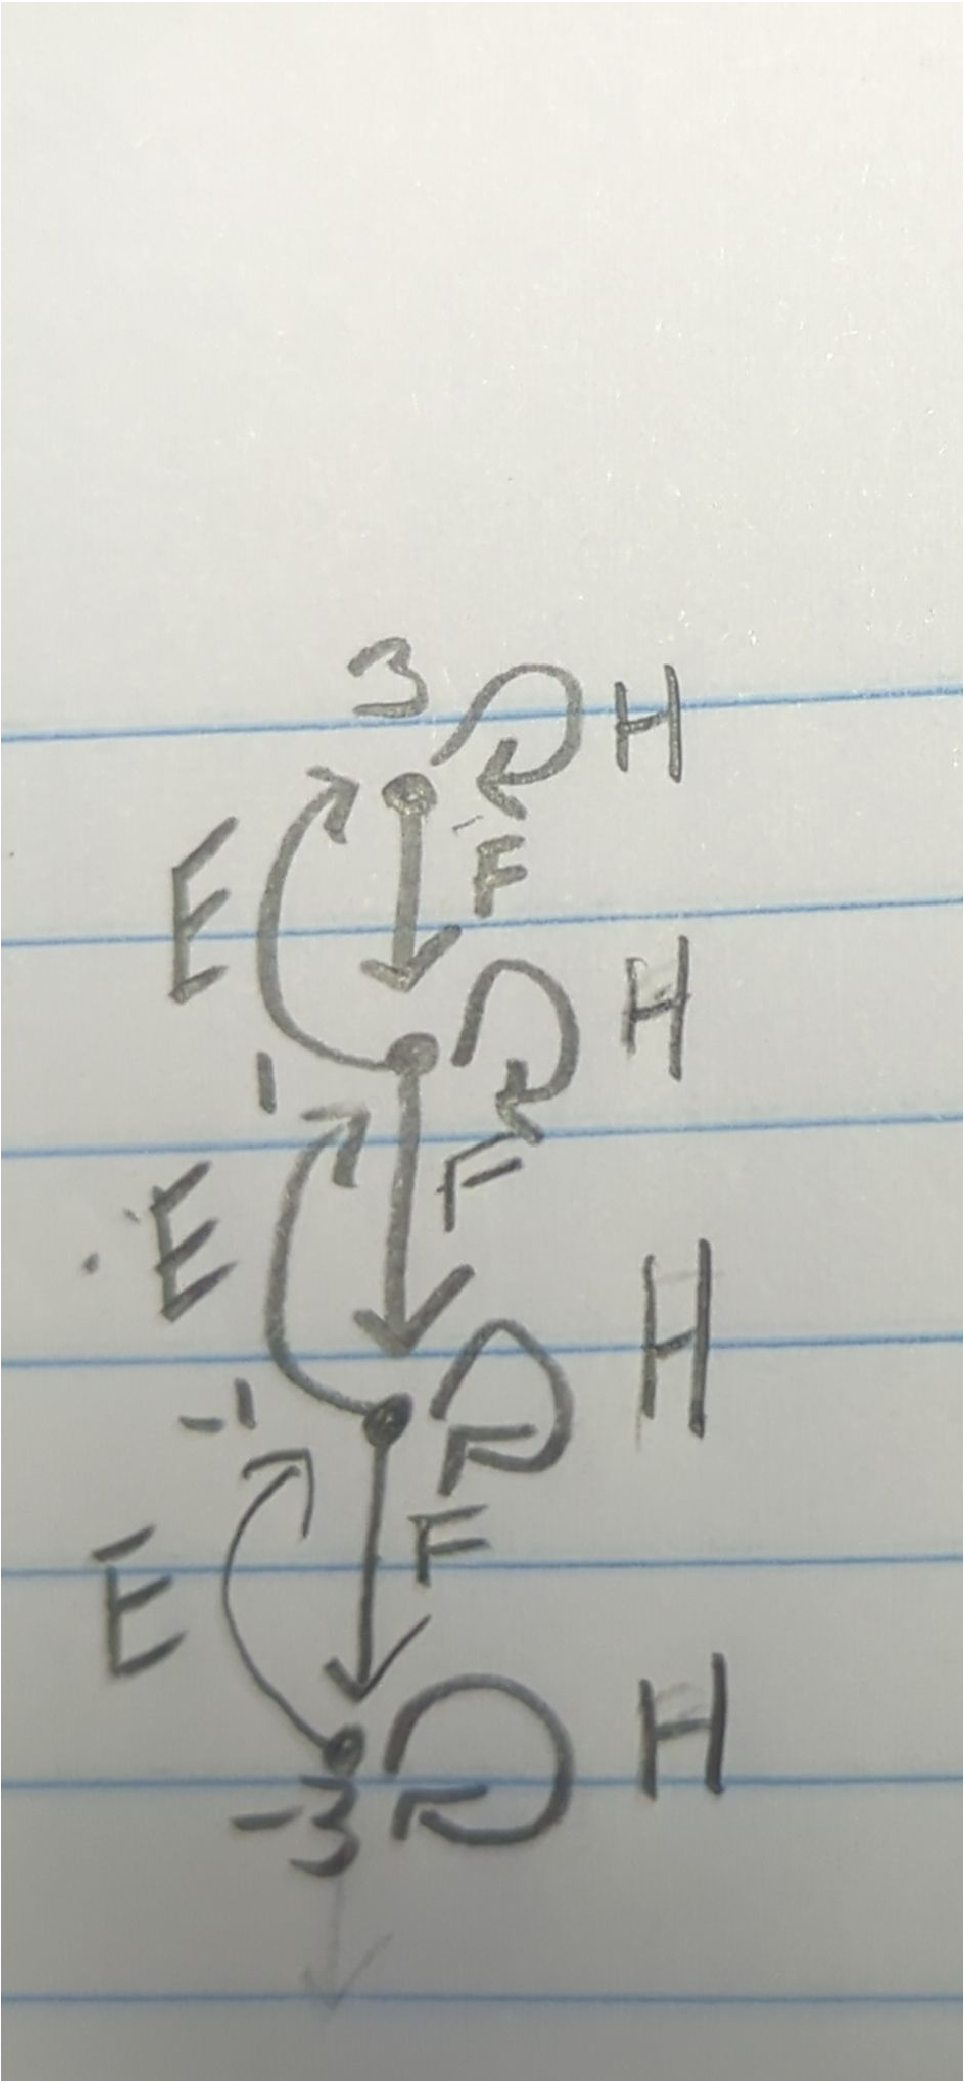
\includegraphics[width=1in]{hw3-1a.pdf}
        %\end{center}
        % 
        \item[(b)] % 3 points
        Consider the representation $\rho:\mathfrak{sl}_2(\C)\ra\mathfrak{gl}_2(\C)=M_{4\times 4}(\C)$ 
        where we will fix the basis $\{v_3,v_1,v_{-1},v_{-3}\}$ In which case we know that we must map to matrices of the form
        \[F\mapsto\begin{bmatrix}
            0&0&0&0\\
            a&0&0&0\\
            0&b&0&0\\
            0&0&c&0
        \end{bmatrix}\]
        \[E\mapsto\begin{bmatrix}
            0&d&0&0\\
            0&0&e&0\\
            0&0&0&f\\
            0&0&0&0
        \end{bmatrix}\]
        \[H\mapsto\begin{bmatrix}
            3&0&0&0\\
            0&1&0&0\\
            0&0&-1&0\\
            0&0&0&-3
        \end{bmatrix}\]
        Furthermore we can use the first requirement of part $c$ that $[\rho(E),\rho(F)]=\rho(H)$ to find that $a=f=3$, $c=d=1$ and $b=e=2$ is a solution, giving
        \[F\mapsto\begin{bmatrix}
            0&0&0&0\\
            3&0&0&0\\
            0&2&0&0\\
            0&0&1&0
        \end{bmatrix}\]
        \[E\mapsto\begin{bmatrix}
            0&1&0&0\\
            0&0&2&0\\
            0&0&0&3\\
            0&0&0&0
        \end{bmatrix}\]
        \[H\mapsto\begin{bmatrix}
            3&0&0&0\\
            0&1&0&0\\
            0&0&-1&0\\
            0&0&0&-3
        \end{bmatrix}\]\\
        
        \item[(c)] % 1 point
         We can now check explicitly that the above map is a representation with matlab 
        \begin{center}
            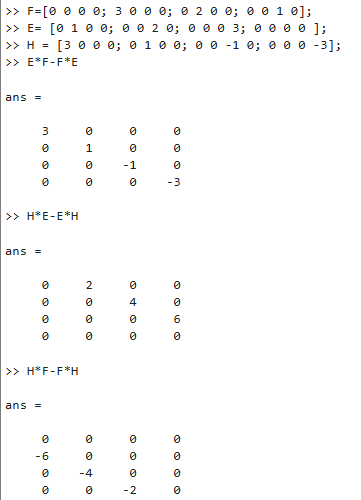
\includegraphics[width=3in]{hw3-1c.png}
        \end{center}
            
    \end{itemize}
    \item[(3)] % 3 points 
    First notice that the formal character of $V^2$ is $\rchi_{V^2}(q)=q^2+1+q^{-2}$
    And 
    \begin{align*}
        \rchi_{(V^2)^{\otimes 3}}(q)&=(\rchi_{V^2}(q))^3\\
        &=(q^2+1+q^{-2})^3\\
        &=q^6+3q^4+6q^2+7+6q^{-2}+3q^{-4}+q^{-6}\\
        &=(q^6+q^4+q^2+1+q^{-2}+q^{-4}+q^{-6})+2(q^4+q^2+1+q^{-2}+q^{-4})+3(q^2+1+q^{-2})+1\\
        &=\rchi_{V^6}(q)+\rchi_{V^4}(q)+\rchi_{V^4}(q)+\rchi_{V^2}(q)+\rchi_{V^2}(q)+\rchi_{V^2}(q)+\rchi_{V^0}(q)
    \end{align*}

    Meaning $(V^2)^{\otimes 3}=V^6\oplus V^4\oplus V^4\oplus V^2\oplus V^2\oplus V^2\oplus V^0$\\


    \item[(4)] % 5 points
    Consider the Tensor product $V^n\otimes V^m$, we will assume WLOG that $n\geq m$.
    Let the vectors $v_n,v_{n-2},\dots, v_{-2}$ be the weight vectors of $V^n$ and $w_m,w_{m-2},\dots w_m$ be 
    the weight vectors of $V^m$.
    Notice that for $k=0,\dots,m$ a vector in the tensor product of the form 
    \[v_{n-2k}\otimes w_m-v_{n-2k+2}\otimes w_{m-2}+\dots + (-1)^{k}v_{n}\otimes w_{m-2}=\sum_{i=0}^{k}(-1)^{i}v_{n-2(k-i)}\otimes w_{m-2i}\]
     is a highest weight vector with weight $n+m-2k$.
     To see this notice that 
     \begin{align*}
        E(\sum_{i=0}^{k}(-1)^{i}v_{n-2(k-i)}\otimes w_{m-2i})&=\sum_{i=0}^{k}(-1)^{i}E(v_{n-2(k-i)}\otimes w_{m-2i})\\
        &=\sum_{i=0}^{k}(-1)^{i}(v_{n-2(k-i)+2}\otimes w_{m-2i}+v_{n-2(k-i)}\otimes w_{m-2i+2})
     \end{align*}
    And notice that this is a telescoping series, so the only terms remaining in the sum are 
    $v_{n-2k}\otimes w_{m+2}$ and $v_{n+2}\otimes w_{m-2k}$ but $w_{m+2}=E(w_{m})=0$ and likewise 
    $v_{n+2}=E(v_{n})=0$ and so the entire sum is $0$, meaning these vectors are in fact highest weight.

    Now we will determine the weight of these vectors, so notice that
    \begin{align*}
        H(\sum_{i=0}^{k}(-1)^{i}v_{n-2(k-i)}\otimes w_{m-2i})&=\sum_{i=0}^{k}(-1)^{i}H(v_{n-2(k-i)}\otimes w_{m-2i})\\
     &=\sum_{i=0}^{k}(-1)^{i}((n-2(k-i))v_{n-2(k-i)}\otimes w_{m-2i}+(m-2i)v_{n-2(k-i)}\otimes w_{m-2i})\\
     &=\sum_{i=0}^{k}(-1)^{i}(n-2(k-i)+m-2i)v_{n-2(k-i)}\otimes w_{m-2i}\\
     &=(n+m-2k)\sum_{i=0}^{k}(-1)^{i}v_{n-2(k-i)}\otimes w_{m-2i}
    \end{align*}
     showing that for each $k$ we have a weight vector with weight $n+m-2k$

     The last thing to check is that these are all the hightest weight vectors, which we will do by counting dimensions. 
     For each $k$ the corresponding vector with weight $n+m-2k$ 
     gives a chain of length $n+m-2k+1$. This means if we sum the number of weight vector 
     in all of the chains we would have a total of $(n+1)(m+1)$ linearly independent vectors, 
     and because the dimension of $V^n\oplus V^m$ is $(m+1)(n+1)$ there can not be any additional chains
     and so there cant be any additional highest weight vectors. This gives is the Clebsch-Gordan rule because the irreducible we formed from each chain are exactly
     $V^n\oplus V^m=V^{n+m}\oplus V^{n+m-2}\oplus\dots\oplus V^{n-m}$


     \item[(5)] % 3 points
     Let $w=w_1w_2\dots w_n$ be a word of $1$s and $2$s that is ballot. 
     Meaning every suffix has at least as many $1$s as $2$s. Notice that this 
     means that for every suffix, every $2$ will be paired with a $1$. 
     This means that there are no unpaired $2$s Applying $E$ would then result in $0$.
     Now assume that $w$ is a word that is not ballot. Meaning there is a suffix 
     $w_i\dots w_n$ that contains more $2$s then $1$s. We may assume that 
     $w_i=2$ and this suffix is of minimal length 
     in which case $w_i$ would be the right most unpaired $2$, as there are less 
     $1$s then $2$s 
     in the suffix. This means that $Ew=w_1w_2\dots w_{i-1}1w_{i+1}\dots w_n$ and 
     so $w$ did not represent a highest weight vector.

\end{itemize}

\end{document}

